\documentclass[aps,prb,twocolumn,groupedaddress,nofootinbib,floatfix]{revtex4}
%
\usepackage{graphicx} 
\usepackage{graphics}
%\usepackage{caption}
%\usepackage{subcaption}
%\captionsetup{compatibility=false}
\usepackage{amsmath}
\usepackage{bm}

%\setlength{\skip\footins}{0.3in}
\begin{document}
%
\title{Migration and Segregation in Three Dimensional Cellular Co-cultures: Role of
Differential Cell Adhesion and Elasticity}

%
\author{Daniel Kolbman}
%
% DON'T CHANGE ANYTHING IN THE NEXT FEW LINES OR DELETE BLANK LINES
%
\affiliation{This work was submitted as part of a course requirement for completion of the BS degree in the Physics Program at RIT and, in its current form, does not appear in any publication external to RIT.}
% % PUT YOUR ADVISOR NAME BELOW.  DON'T DELETE ANY LINES
%
\altaffiliation [Rochester Institute of Technology, School of Physics and Astronomy, Faculty Advisor: ]{Moumita Das}

\date{\today}

\begin{abstract} \noindent The biophysics of cell co-cultures, i.e. a binary system of cell populations, is of great interest in many biological processes including formation of embryos, and tumor progression. 
During these processes, different types of cells with different physical properties are mixed with each other, with important consequences for cell-cell interaction, aggregation, and migration. The role of the differences
in their physical properties in their collective behavior remains poorly understood. Furthermore, until recently, most experiments and theoretical models of collective cell migration have focused on two dimensional systems.
Under physiological conditions, however, cells often have to navigate three dimensional and confined micro environments.
I have modelled cell co-culture systems by extending previous two-dimensional Brownian Dynamics simulation of a binary system of interacting, active, and deformable particles to a confined three-dimensional system. I compare results from the model with experiments done by our collaborators.
Findings may provide insights into how the differences in cells' physical properties such as elasticity, propensity for cell-cell adhesion, and self-propulsion speeds of two cell types influence emergent collective properties such as cell aggregation and differential migration experimentally observed in co-cultures of breast cancer cells and healthy breast epithelial cells.  
\end{abstract}

\maketitle

\section{Background and Motivation}

In several biological processes, from the formation of embryos to the formation and progression of tumors, cells with different physical properties are present in close proximity, with important consequences for cell-cell interaction, aggregation, and migration \cite{Lee, Suresh}.
Laboratory cell co-cultures made of two different cell populations are ideal systems to qualitatively and quantitatively study how distinct physical properties of cells can influence such emergent behavior. Here I construct and study a simple proof of concept model of a cell co-culture in three dimensions 
and under confinement to test the hypothesis that differential physical properties of cells can drive segregation and preferential migration in co-cultures.   
The experimental system that motivates this work is a co-culture of breast cancer cells and non-cancer breast epithelial cells. 
This system provides an excellent platform because of the characteristic differences between the two cell types \cite{Lee,Mingming}. 
For example, the nucleus and cytoplasm of breast cancer cells have been found to have relatively low elastic moduli compared to their non-cancerous counterparts \cite{Lee}. 
As a result, the cancer cells are much more deformable. Recent experiments suggest that this mechanical mismatch may play a key role in cancer cell migration through a healthy
cell population \cite{Lee}. 

Until recently, most experiments and models of cell co-cultures have focused on two dimensional systems, with limited application to physiological conditions\cite{Jong}.
Recently, new techniques for observing co-cultures in three dimensions have become available\cite{Alessandri}.
Accordingly, I seek to formulate a minimal model of co-culture cell mechanics in three dimensions by extending previous two dimensional simulations of binary systems of deformable and active colloids\cite{Butcher}.
Using an integrated modelling and experimental approach, I aim to characterize the role of differences in physical properties such as cell stiffness, cell-cell adhesion, and self-propulsion in  aggregation and migration in co-cultures of breast cancer cells and non-cancerous cells in three dimensions.
Furthermore, I focused on a confined system to better recreate the physiological and experimental systems our collaborators are studying.
From a physics perspective, I study the interplay of cell mechanics, and statistical mechanics in cell migration in a confined binary system in three dimensions.
The main ingredients of this model are discussed below.\\


\subsection{Differential physical properties of binary cell populations: mechanical stiffness, cell-cell adhesion, and self-propulsion of cancer cells Vs. non-cancerous cells}

This computational study seeks to understand the biophysics of a model binary system consisting of two types of cells: breast cancer cells and healthy breast epithelial cells. 
Healthy breast epithelial cells and breast cancer cells, particularly the cell lines MCF-7 and MDA-MB-231 respectively, have been widely studied and their physical properties are well known \cite{Suresh}.
Experimental work involving these two cell types has shown interesting emergent behavior. 
One such phenomenon occurs when cancer cells are introduced to a monolayer of healthy cells.
In this experiment, the cancer cells are observed to have higher migration speed than when in a monolayer consisting solely of other cancer cells \cite{Lee}.
Another interesting behavior observed by experimentalists is the separation of the two cell types \cite{Lu}.
They found that when a co-culture of cancer and healthy cells are confined in a spherical microfluidic droplet, they separate with cancer cells accumulating near the boundaries of the droplet and the healthy cells aggregating in the center \cite{Mingming}.
In addition to the difference in stiffness \cite{Lee}, the adhesion properties of most cancer cells have also been found to be drastically different from that of non-cancerous cells of the same tissue type\cite{Jeanes}.
Most healthy cells adhere to each other via the protein E-cadherin when they come in contact. Cancer cells lack this adhesiveness. Cancer cells further show enhanced self-propulsion (i.e. how fast individual cells can propel themselves by consuming ATP or due to other internal forces in the absence of any other interaction forces), compared to non-cancerous cells of the same tissue type \cite{Suresh}. The differences in the adhesiveness, stiffness, and self propulsion of the two cell types are key ingredients in the our model.


\subsection{Cell Migration in Three Dimensions}

Previously several experimental and theoretical studies have addressed various aspects of cell migration in two dimensions, including protrusion, adhesion, and retraction at the level of single cells, and collective motion at the multicellular level \cite{}.
However, the {\it in vivo} environment for a crawling cell is typically a three-dimensional environment, consisting of the extracellular matrix (ECM) and surrounding cells.
Recent experiments show increased migration rates of cells in three-dimensional matrices as opposed to two-dimensional surfaces \cite{Cukierman}.

\subsection{Role of Confinement}

Ongoing experiments in the laboratories of our collaborators Dr. M. Wu and Dr. M. Ma involve observing co-cultures inside spherical capsules with diameters of the order of several hundred micro-meters 
and containing hundreds of cells\cite{Alessandri} (See FIG. \ref{fig:capsule}). Given that confinement and finite system size can have important consequences for the statistical mechanics and collective 
properties of the cell-culture, it is vital to account for them in the model. The spherical capsules in the experiments mentioned above have an inner diameter of $50-700\mu m$ and an outer diameter of $400-7000\mu m$ \cite{Mingming}.
The cells are present inside the inner capsule and have dimensions of the order of $\sim 10\mu m$.
The region between the inner and outer diameters is occupied by a dense gel layer that the cells can not penetrate.
The outside of this layer is coated such that cells will not adhere to this layer upon contact. \\

\begin{figure}
  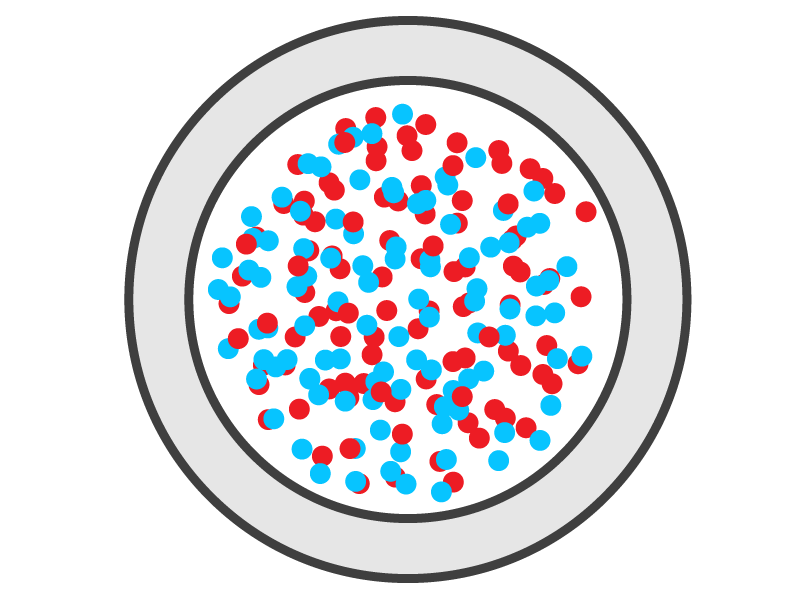
\includegraphics[width=3in]{images/Fig1.png}
  \caption[capsule]
   {A cross section schematic of a spherical capsule enclosing a binary mixture of 
   cells.}
   \label{fig:capsule}
\end{figure}


\section{Model}

\begin{figure}
  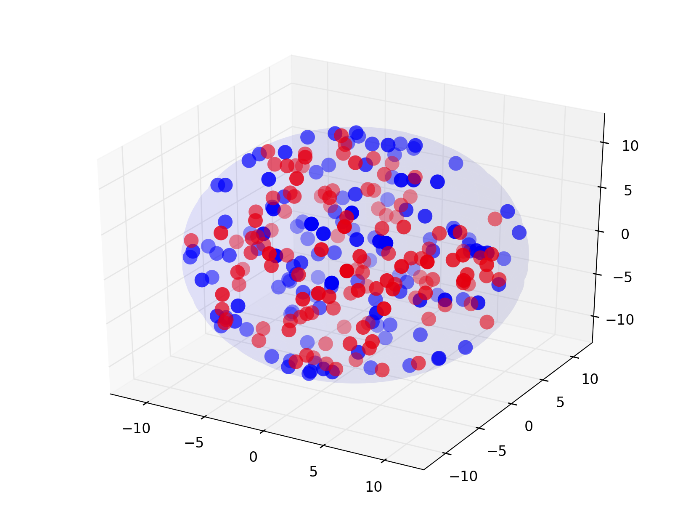
\includegraphics[width=1.0\columnwidth]{images/3dconf.png}
  \caption[3dconf]
    {A sample initial configuration of a confined three dimensional co-culture system. The blue spheres represent the cancer cells, and the red spheres represent the healthy cells
    (this color scheme is followed throughout this paper). Note that the two cell types are randomly and isotropically distributed. The two types of cells are of the same size, and the sizes are not shown
    to scale in the figure.}
   \label{fig:3dconf}
\end{figure}

I study the collective dynamics of this system using an active Brownian Dynamics simulation. Brownian dynamics is ideal for this system as cells behave like Brownian particles: their dimensions and timescale of motion are much larger than that of the particles of the surrounding medium in which they are suspended and in equilibrium  their motion is diffusive.
In addition, the system is ``active" because cells can generate forces by consuming ATP and propel themselves.
A simple model of a homogeneous monolayer of such active particles consists of a two dimensional system of interacting colloidal particles that are also each active, i.e. self-driven \cite{FilyMarchetti,RednerBaskaran}. 
Such models have been previously used to study swarming  behavior \cite{Vicsek} in birds, insects, and fish.
This approach  has recently been combined with cell mechanics and applied it to a binary population of cells, to study the collective mechanics and dynamics in cell co-cultures characterized by a difference in cell stiffness \cite{Butcher}.
This study found that mechanical mismatch in co-cultures can have important consequences cell migration, and can lead to enhanced motility for more deformable cells\cite{Butcher}, 
in agreement with the Lee and coworkers \cite{Lee}. In the current project, I have extended this model to a three-dimensional system, included cell-cell adhesion, and further added the presence of a confining sphere to mimic the experimental set-up used by our collaborators \cite{Mingming}. 

\begin{figure}
  \begin{subfigure}{\columnwidth}
    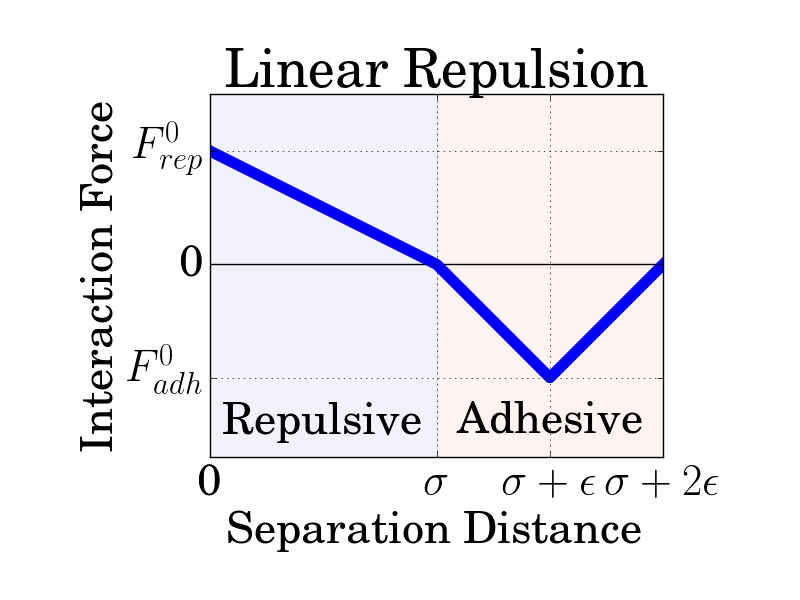
\includegraphics[width=1.0\columnwidth]{images/interaction.png}
      \caption{Schematic diagram of the qualitative form of the two part contact interaction force. When two cells push into each other such that the separation between their centers is less than the diameter of the cells, there is a Hookean, elastic restoring (repulsive) force. Neighboring cells that have not pushed into each other, but are within a certain close distance of each other, may experience an adhesive force. The strengths of the forces are determined by the prefactors $F_{rep}^0$ and $F_{adh}^0$. The effective separation between cells for adhesive force to be non-zero is set by a contact distance, $\epsilon$  in the model (Not illustrated to scale).}
  \end{subfigure}
  \begin{subfigure}{\columnwidth}
    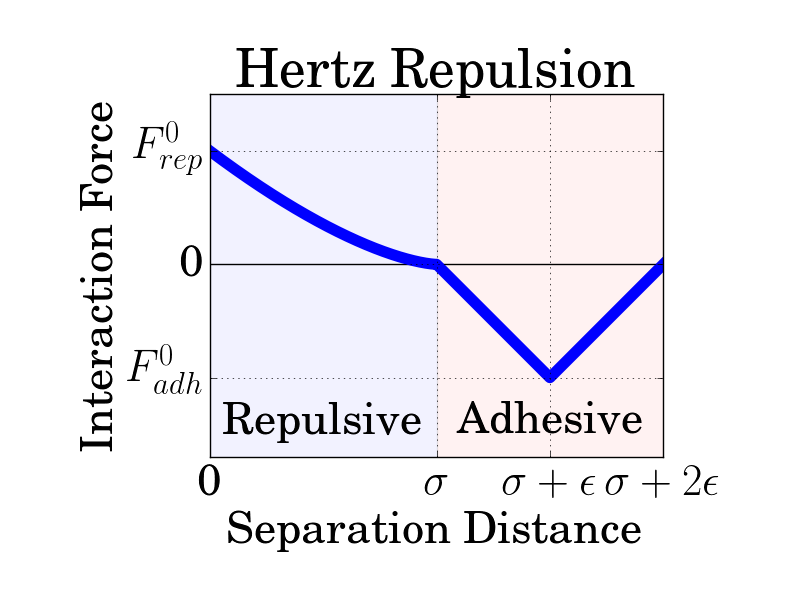
\includegraphics[width=1.0\columnwidth]{images/hertz.png}
    \caption{Schematic diagram of the qualitaticve form of the two part contact interaction force with the Hookean interaction replaced with a Hertzian interaction.}
  \end{subfigure}
  \label{fig:interaction}
\end{figure}

My model of the co-culture is made of two types of active Brownian particles representing the cancer and healthy cells (See FIG. \ref{fig:capsule}). 
The cells only interact with each other when they come into contact.
The contact interaction between cells is of two types.
First, when cells come into contact and push against each other, depending on their mechanical stiffness they will respond with different forces; this interaction is modeled as an elastic repulsive interaction.
For the non-cancerous (stiff) cells, there further exists a cell-cell adhesion, modeled here as an attractive interaction at contact.
The cancer cells do not have this adhesion.
The strengths of the interactions are tuned to mimic physiological conditions, where I use a stiffness of $2000 Pa$ for the stiff  (healthy) cells and $667 Pa$ for the soft (cancer) cells \cite{Lee},
and a diffusion constant of $\sim 1.8 \mu m^2 /min$ for both cell types \cite{Mingming}.
Both cell types have the same diameter  $\sigma = 15$ $\mu m$.
The particle positions evolve according to the overdamped Langevin equations \cite{Lemons,RednerBaskaran,FilyMarchetti,Butcher}: 

\begin{equation}
  \bm{\dot{\bm{r}_i}} = \frac{1}{\gamma}\bm{F}_{int}(\bm{r}_i) + v_p\hat{\bm{v}}_i+\sqrt{2D}\eta_i^T
\end{equation}

\begin{equation}
  \dot{\theta}_i=\sqrt{2D_r}\eta^R_i
\end{equation}

Where $F_{int}$ is the total interaction forces on the cell from adhesion and repulsion.
The variables $\bm{r}_i$ and $\dot{\bm{r}}_i$ are the position and velocity of the i\textit{th} particle, respectively.
The constant $\gamma$ is the damping coefficient of the fluid used. It is related to the
diffusion constant, $D$, by $D=\frac{k_BT}{\gamma}$, where $k_B$ is the Boltzman constant and $T$ is temperature and has been set to $298$ Kelvin. 
The variable $v_p$ is the magnitude of propulsion and is $\sim 100 \mu m/hr$ in my experiments, and $\bm{\hat{v}}_i$ is the direction of propulsion, $\bm{\hat{v}_i}=(\cos \theta_i, \sin \theta_i)$.
The noise $\eta^T$ represents fluctuations in translational motion and account for collisions with smaller fluid particles, while
$\eta^R$ is the rotational noise to simulate fluctuations in the direction of travel from ATP use by cells. Both types of noise follow Gaussian statistics, and satisfy the fluctuation dissipation theorem \cite{}.

\begin{equation}
\left\langle \eta_i(t)\eta_i(t')\right\rangle = 0 
\end{equation}
\begin{equation}
\left\langle \eta_i(t)\eta_j(t')\right\rangle = \delta_{ij} \delta(t-t')
\end{equation}

% Dimension stuff %

We define $k_BT$ and $\sigma$ to be our units of energy and length, respectively, and define 
unit time as $\tau = \frac{\sigma^2}{D}$. These units are used to non-dimensionalize 
energy, length, and time scales in the simulation. Total particle volume fraction is set to $70\%$ unless mentioned otherwise, and 
the Peclet number of the system, defined as $Pe= v_p \tau/\sigma$, and is chosen to be 12 in the simulations.
In the experimental system it is  $\sim 12.5$. 
The chosen particle volume fraction and Peclet number ensure a system that is not jammed but close to confluence.
Furthermore, in the low-Reynolds number regime \cite{RednerHagan}, the rotational diffusion $D_r$ is related to the translational 
diffusion $D$ as $D_r= 3 D /\sigma^2$, I have added an additional prefactor $<1$ to account for a smaller
rotational diffusion due to the presence of the extracellular microenvironment felt here in an average sense.


% Interaction forces %

The interaction forces are important for investigating how the elasticity and adhesivity of cells affects their migration and segregation. For non-cancerous cells, 
I have modeled the stiffness of the cells using (i) a simple Hookean spring potential, and (ii) a Hertz interaction potential, while I use a `V' well to model the adhesion (See FIG. \ref{fig:interaction}). 
The result is particles that will desire to be close together, while resisting overlap. Cancer cells have qualitatively similar (but weaker) elastic repulsion, and not do not show 
cell-cell adhesion because of the lack of the protein E-cadherin \cite{Jeanes}. 


For two cells whose centers are separated by a distance $r$, I first modeled the elastic repulsion by a  Hookean interaction as follows, with amplitude $F^0_{rep}$ determined phenomenologically.
 
\begin{equation}
  F_{rep}(r) = F^0_{rep} \left\{ 
    \begin{array}{lr}
      1-\frac{r}{\sigma} &, r < 0\\
      0 &, r \ge \sigma
    \end{array}
  \right.
  \label{eq:frep}
\end{equation}

Next, we carried out the simulations with the more physiologically realistic Hertz interaction force for non-adhesive contact mechanics between two deformable spheres (cells) given by \cite{}:

\begin{equation}
  F_{rep}(r) = F^0_{rep} \left\{ 
    \begin{array}{lr}
      (1-\frac{r}{\sigma})^{3/2} &, r < 0\\
      0 &, r \ge \sigma
    \end{array}
  \right.
  \label{eq:frep}
\end{equation}

The force $F^0_{rep}$ is given by $(2 \sqrt/3) E^* \sigma^2$ where $E$ is the effective Young's modulus given by $1/E^*=1/E_1 + 1/E_2$, $E_1$ and $E_2$ being the Young's moduli of the two cell types. 


The magnitude of the adhesive force is given by:

\begin{equation}
  F_{adh}(r) =F^0_{adh} \left\{
    \begin{array}{lr}
      0 &, r \le \sigma \\
      \frac{|r - (\sigma+\epsilon)|}{\epsilon}-1 &, \sigma < r < \sigma+2\epsilon
    \end{array}
  \right.
  \label{eq:fadh}
\end{equation}

The forces act along the separation between the center of the two particles. The force amplitudes  $F^0_{rep}$ and $F^0_{adh}$ depend on the species of the particle.  The parameter $\epsilon$ is half the phenomenological lengthscale over which the non-cancerous cells show cell-cell adhesion (See FIG. \ref{fig:interaction}). 


% Physical system (Boundaries, packing fraction) %

\subsection{System Conditions}
`Hard' barrier boundaries have been imposed on the system to imitate the conditions of confining microfluidic shells used in the experiments \cite{Mingming}. 
This means that particles may move along or within a specified radius, but are restricted from moving outside of it.
I begin each simulation with an initial configuration where the two species are intermixed and the cells are randomly and uniformly distributed inside of the confining sphere.
The size of the system is dependent on the packing fraction of the system.
In my simulations, I have studied multiple packing fractions from $\phi=0.4$ to $\phi=0.9$ for each cell type. Unless otherwise mentioned, the results shown here were obtained
for a binary system with packing fraction $\phi=0.7$ for each species which is where active colloidal systems have been studied in the past\cite{RednerBaskaran}, and found to form a nearly confluent system at long times. 
See FIG. \ref{fig:3dconf} for a sample three dimensional system.


% Technical stuff %
\section{Numerical Methods}

\begin{figure}
  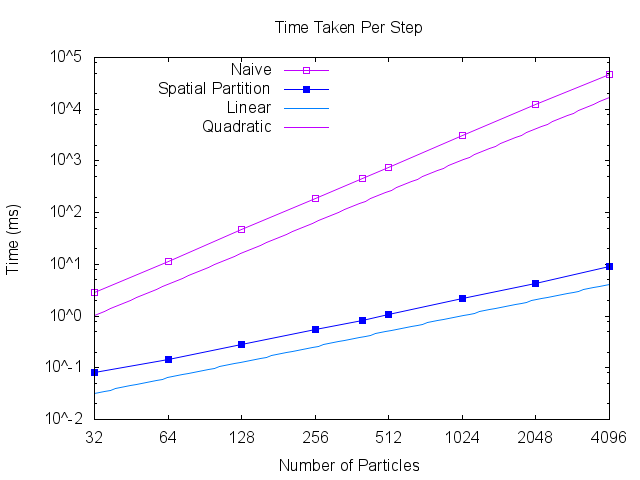
\includegraphics[width=\columnwidth]{images/compare.png}
  \caption{Comparison between naive and spatial hashing collision methods}
  \label{fig:compare}
\end{figure}

The dynamics simulations are computed in Julia, a high-performance, dynamic 
programming language for scientific computing \cite{Bezanson1,Bezanson2}.
The code was documented and published using Sphinx \cite{RTD} and the source released on Github \cite{github}.

The simulations use a forward Euler method to integrate with time steps between $10^{-4}\tau$ and $10^{-6}\tau$.
The model is heavily dependent on near-range interactions with other particles in a many body system.
To reduce run time, spatial hashing techniques for collision detection were used \cite{Muller}.
This works by dividing the simulation space into discrete blocks, iterating over all blocks in the system, and considering partcle pair interactions only between the current and neighboring blocks.
The result was a model that scaled linearly with the number of particles rather than with the number of particles squared in a naive collision model (See FIG. \ref{fig:compare}).

Many identical simulations were run ten or more times to create ensemble averages for the quantities I was measuring.
To reduce runtime when computing many simulations for desired parameter set, simulations were performed in parallel on a computing grid with each CPU core handling one simulation at a time.


One common measurement made by experimentalists on tracking data of cells is the mean squared displacement (MSD) averaged over all cells of a given type.
It is given as:

\begin{equation}
  MSD \equiv <(x(t) - x(0))^2>
\end{equation}

I also use this measurement to analyze the motility of the different cell types in the simulation.

The differential adhesion hypothosis is that the intercellular adhesion varies depending on the presence of cadherins \cite{Foty}.
When the the level of cadherin expression is increased, it is found that the size of the aggregating clumps increased. 
To measure the size of the cluming that occured in the model, I used DBSCAN, a common clustering algorithm used in machine learning \cite{Ester}. 
It works by choosing random points in the data, then searching for neighboring points a specified distance away.
This process repeats on all neighboring points found in the initial point.
The result is a number of clusters of different sizes.
For results here, it was chosen that any point $1.1\sigma$ from another point was to be considered a neighbor.

\section{Results}


\subsection{Brownian Diffusion}
According to Einstein's theory of brownian motion, it is expected that the mean
squared displacement of a particle undergoing Brownian motion in three dimensions should evolve proportional to the time, with a proportionality constant $6 D$ \cite{}, where $D$ is the diffusion constant.
In the non-dimensionalized model, this constant pre-factor should be $6$. This fact was used to confirm that the dynamics of the simulation were working properly.
To test this, all interaction and propulsive forces were turned off and the system was evolved only under brownian forces.
Ten identical simulations were run and averaged to produce FIG. \ref{fig:brownianMSD}. The slope is very nearly the expected value and is expected to be exact for larger numbers of trial runs and larger system sizes.


\begin{figure}
  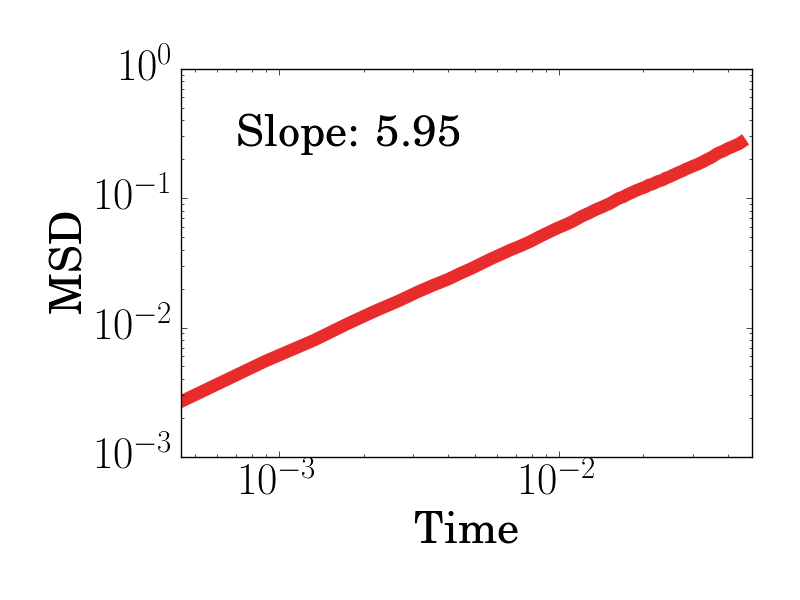
\includegraphics[width=\columnwidth]{images/brownianMSD.png}
  \caption[brownianMSD]
    {MSD for a single species system under only brownian forces. The MSD evolves nearly as $6Dt$ as expected from Einstein's theory of brownian motion. The time is expressed in units of $\tau$, and MSD is expressed in units of $\sigma^2$ defined earlier.}
  \label{fig:brownianMSD}
\end{figure}

\subsection{Segregation}

Next I focused on the segregation of the cancer cells from the non cancer cells
observed in ongoing experiments by our collaborators Drs. Ma and Wu. 
They have found that, starting with a randomly distributed mixture of breast cancer cells,
and non-cancerous breast epithelial cells inside the spherical microfluidic capsule, over long times
(of the order of a week\cite{Lu}), the two cell types phase separate. The healthy cells assemble in the the center of capsule,
while the cancer cells collect near the boundary and form an outer shell. By using parameters similar to those 
in the experiments, I was able to qualitatively replicate this using our model.


We start with an initial random and uniform distribution of the two cells types consisting of  
equal number of cells for each type. As described before, the cancer cells experience an elastic
repulsion that is much weaker than that experience by the non-cancerous cells.
Furthermore, cancer cells experience a self-propulsive force but no cell-cell adhesion, while non-cancerous cells experience cell-cell adhesion, but no self-propulsion.
There is no cell-cell adhesion between cancer cells and non-cancerous cells.
Under these conditions, the system was allowed to evolve (See FIG. \ref{fig:separation}).
The system separates from its initial (random) state so that the cancer cells move toward the boundary.

\begin{figure}
  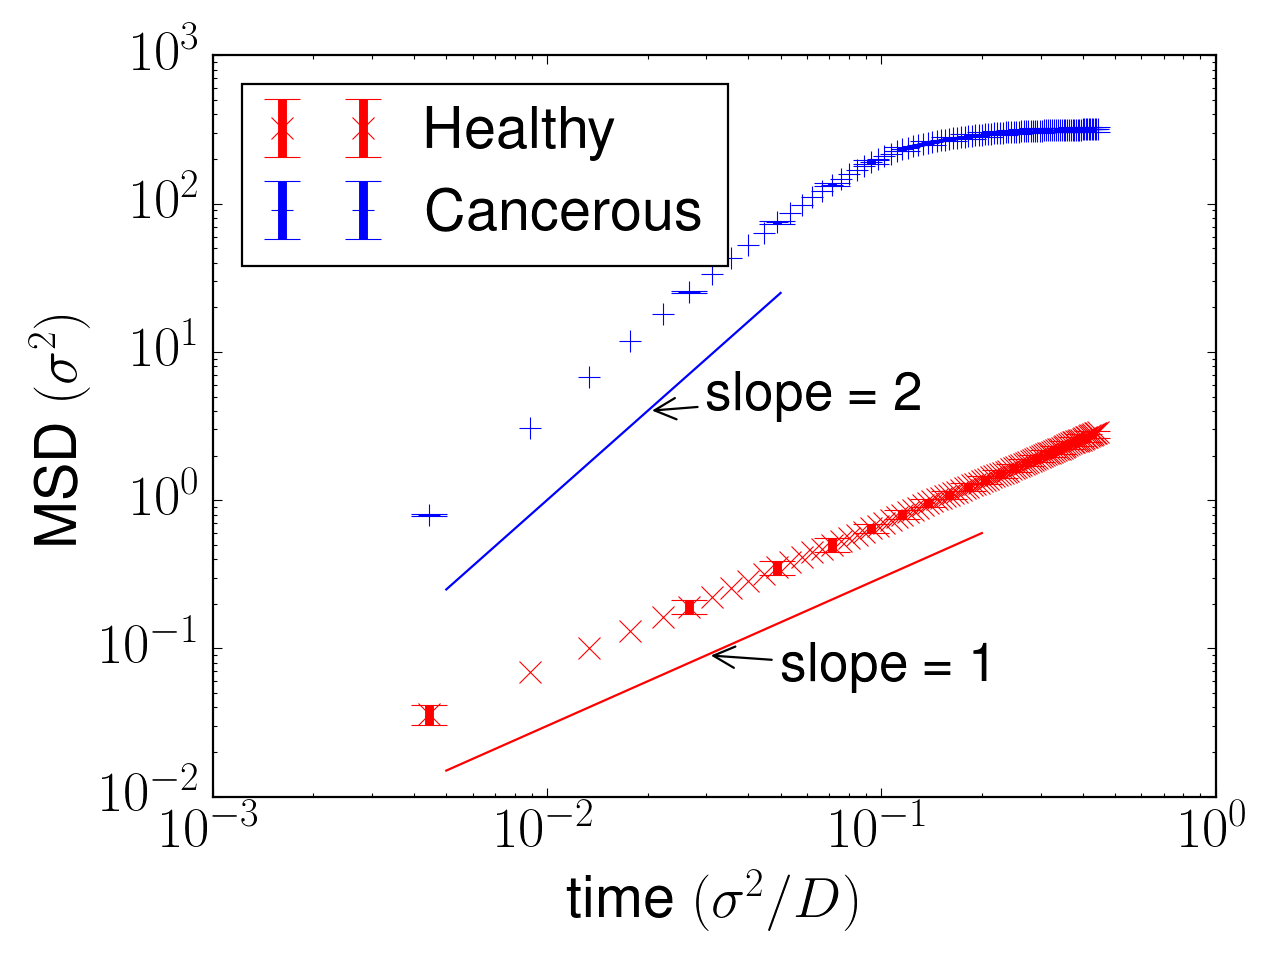
\includegraphics[width=\columnwidth]{images/cocultureMSD.png}
  \caption[cocultureMSD]
    {The short timescale MSD for a co-culture, cancer-healthy cell system. The cancer cells
    are observed to be much more motile than the healthy cells, and their MSD has a larger slope. The time is expressed in units of $\tau$, and MSD is expressed
    in units of $\sigma^2$ defined earlier. The parameters for the stiffness and diffusivity used are obtained from experiments as described in the text.  This result is
    similar to those of the two dimensional case\cite{Butcher}.}
  \label{fig:cocultureMSD}
\end{figure}

\begin{figure}
  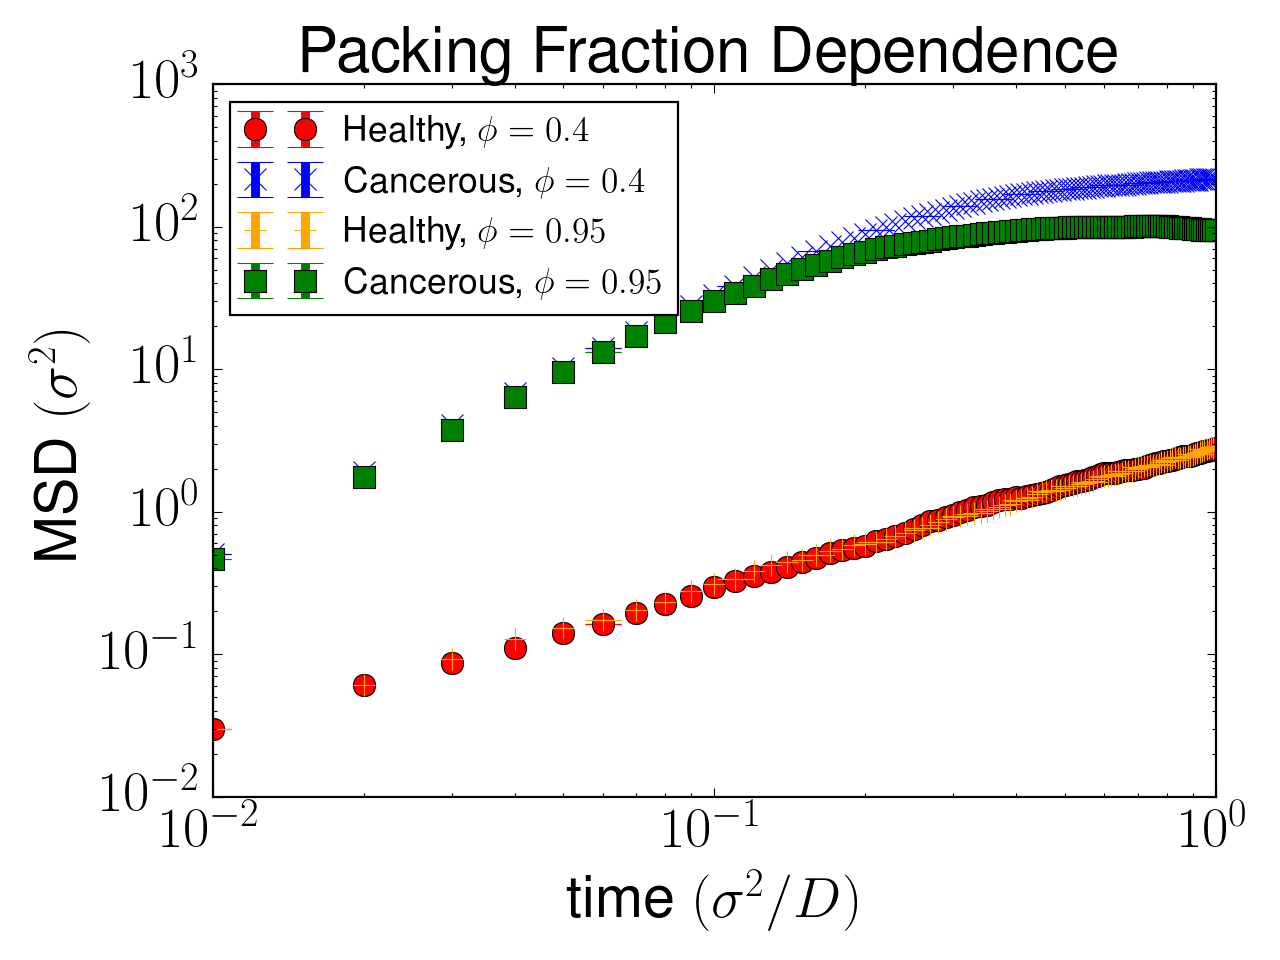
\includegraphics[width=1.0\columnwidth]{images/phi_both.png}
  \caption{The pacing fraction at two extremes: $\phi=0.4$ (top) and $\phi=0.95$ (bottom).}
  \label{fig:phi}
\end{figure}

\subsection{Differential Migration}
One case that was investigated closely in the two-dimensional model was a co-culture system with healthy, adhesive cells, and cancerous, propulsive cells with an elasticity difference of one order.
As in the two-dimensional case, it was found that in the three dimensional co-culture, the cancer cells migrated faster than the healthy cells.
This is represented by the larger slope of the mean squared displacement vs time (ballistic motion) for the cancer cells compared to the healthy cells (diffusive motion). See FIG. \ref{fig:cocultureMSD}.

\subsection{Towards constructing a phase diagram}

Due to the computational intentsity of the simulation, a system comparable to the systems produced in the lab consisting of millions of cells is not feasible.
Instead, a much smaller system (512-1024 cells) was needed to produce results in a reasonable fashion. I ran the model under similar conditions for different quantities of cells to determine what considerations to make when comparing my model to experimental results from our collaborators.
One goal of this project is to construct a multi-dimensional phase diagram with respect to several parameters.
A full phase diagram is outside the scope of this report for lack of time, though I have collected and analyized cases with independantly varying parameters.
Below I have described my observations of the dependence of the emergent properties of the system on important constitutive  physical properties of the cells that can form the axes of the planned diagram.

\subsubsection{Packing Fraction}

\begin{figure*}
  \begin{subfigure}{\columnwidth}
    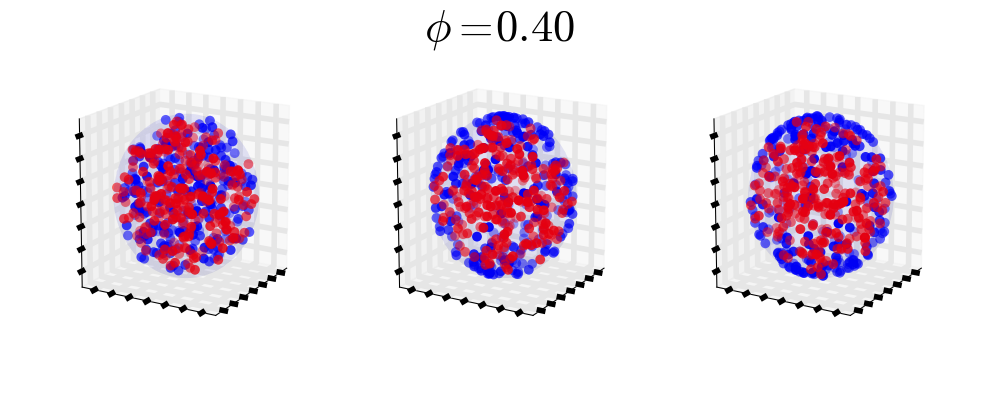
\includegraphics[width=1.0\columnwidth]{images/configs_40.png}
  \end{subfigure}
  \begin{subfigure}{\columnwidth}
    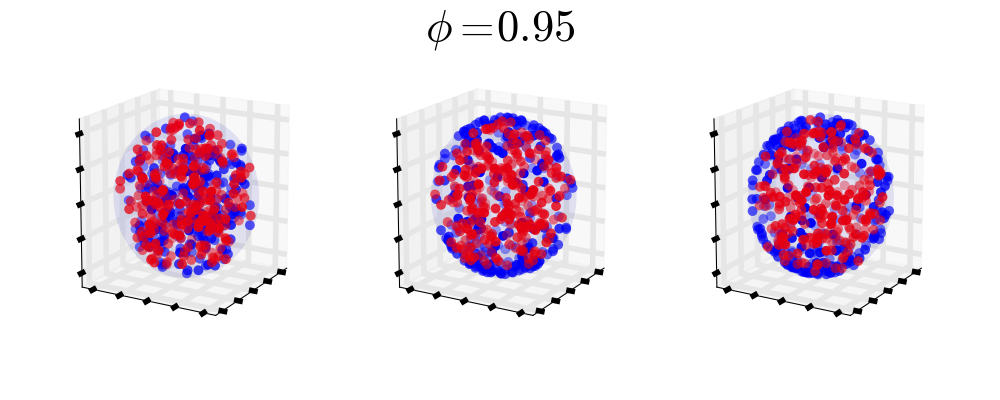
\includegraphics[width=1.0\columnwidth]{images/configs_95.png}
  \end{subfigure}
  \caption{The system configuration for two packing fraction extremes, $\phi=0.4$ and $\phi=0.95$}
  \label{fig:packing_configs}
\end{figure*}

The critical packing fraction for solid (hard)  spheres where the system becomes jammed is $0.74$.
Given that the model consists of deformable spheres as opposed to solid spheres, it was expected that the reach a critical packing fraction above $0.74$ and show significantly reduced motility in both species.
The model was run for several packing fractions between $0.4$ and $0.95$ by keeping the number of particles fixed and altering the size of the system appropriatly.
The extremely high packing fraction of $0.95$ was expected to be jammed and show very little migration of any cells.
However, results show that there is little effect on the behavior of the system at such high ratios (FIG. \ref{fig:phi}).
When considering snapshots of the system (FIG. \ref{fig:packing_configs}), it can be seen that this is due to the aggregation of the healthy cells.
As a result, there is considerable overlap of cells resulting in a lower effective packing fraction that allows cells the ability to migrate.



\subsubsection{Stiffness}

One motivating hypothesis behind this model was that the difference in cell elasticity caused a mismatch in motility of the two cell species.
The model was run for several different ratios of stiffness between the two cells ranging up to three orders difference between the two.
The resulting behavior, however, did not show any identifiable differences in the system behavior for different ratios of stiffness.
This indicates that the differential stiffness between the cell types is not as significant as the adhesive and propulsive forces in the overall behavior of the system all size.

\subsubsection{Cell-cell adhesion}

There are two parameters that affect the adhesive force of the healthy cells in the model.
The first is the magnitude of the force.
This is the prefactor that scales the force similar to the repulsive force.
The second is the contact distance of the adhesive force, $\epsilon$.
This is how far the bottom of the well is from the edge of the cell (See FIG. \ref{fig:interaction}).

The strength of the adhesive force was varied for the healhy cells from $10$ to $1000$ in the dimensionless units with a contact distance of $0.2$.
The resulting behaviors did not vary significantly with respect to the MSD or clustering of the healthy particles.
The contact distance was also varied with a set adhesive strength of $1500$.
This resulted in many more clusters being formed and a decrease in the motility of the healthy cell species.


\begin{figure}
  \begin{subfigure}{\columnwidth}
    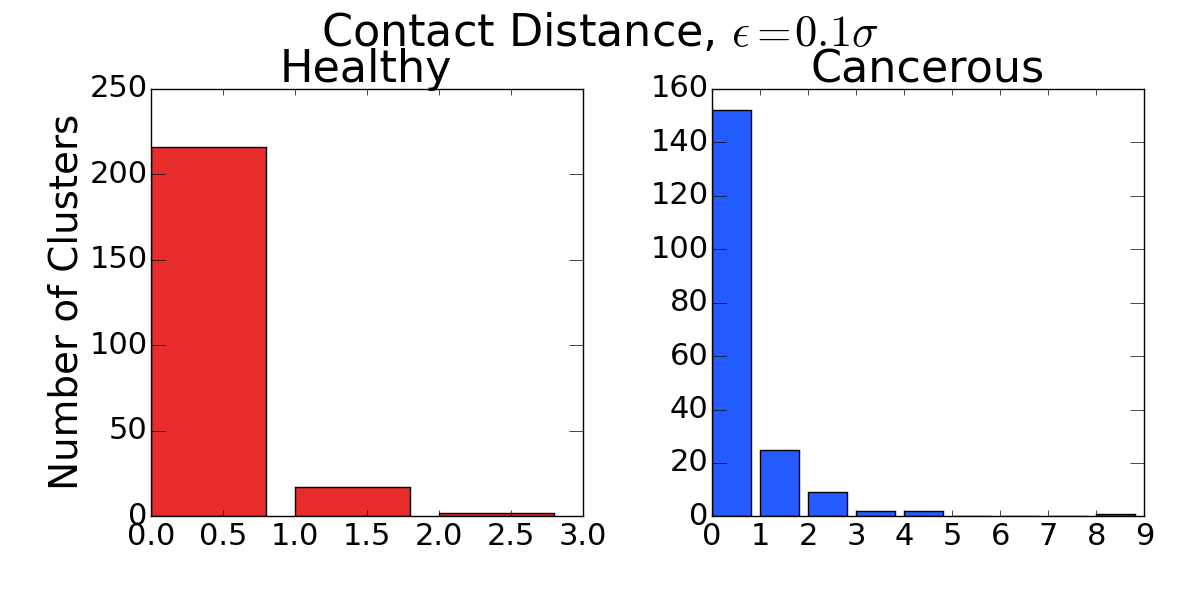
\includegraphics[width=1.0\columnwidth]{images/contact1.png}
  \end{subfigure}
  \begin{subfigure}{\columnwidth}
    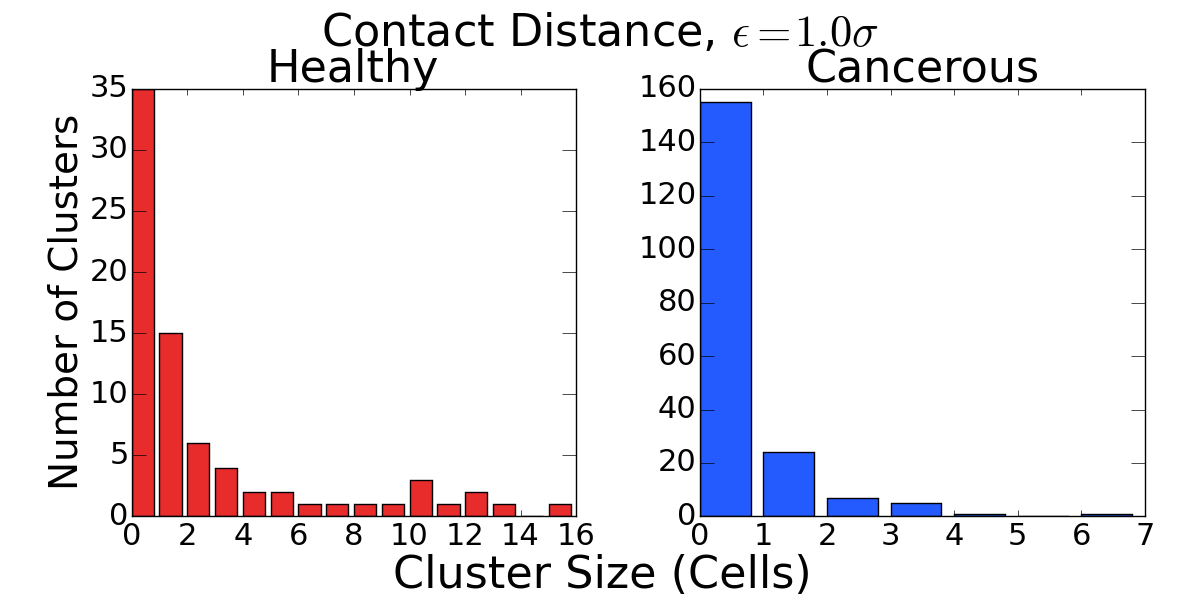
\includegraphics[width=1.0\columnwidth]{images/contact2.png}
  \end{subfigure}
  \caption{Number of clusters for different effective distances of the adhesive force ($\epsilon$).The figure shows only a few small clusters exist for low effective distances ($\epsilon=0.1$) while larger clusters are more likely to exist for larger effective distances ($\epsilon=1.0$).}
  \label{fig:contact}
\end{figure}

\begin{figure}
  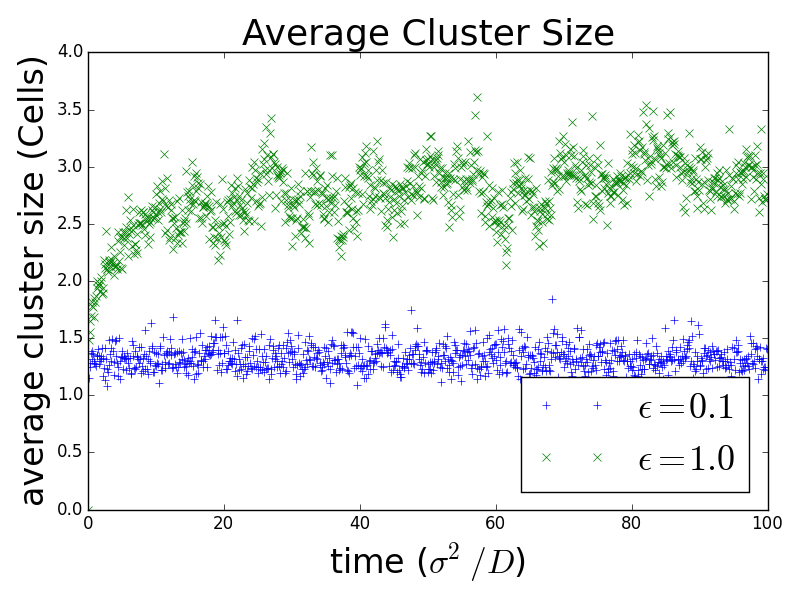
\includegraphics[width=1.0\columnwidth]{images/avg_clusters.png}
  \caption{The average number of clusters as a function of time for two extremes of the effective adhesive contact distance, $\epsilon$.}
  \label{fig:clusters}
\end{figure}


\subsubsection{Self-propulsion speed}

The dependence of the motility on the self-propulsion of the cancer cells in the model was tested by varying the Peclet number.
For a low Peclet number, $Pe=1$, the cancer cells showed only diffuse behavior and did not seperate from the diffusive healthy cells (See FIG. \ref{fig:prop}).
For a high Peclet number, $Pe=1000$, the cancer cells were observed to be more motile than the healthy cells.
These results indicate the seperation behavior is dependent on the activity of the cancer cells.

\begin{figure}
    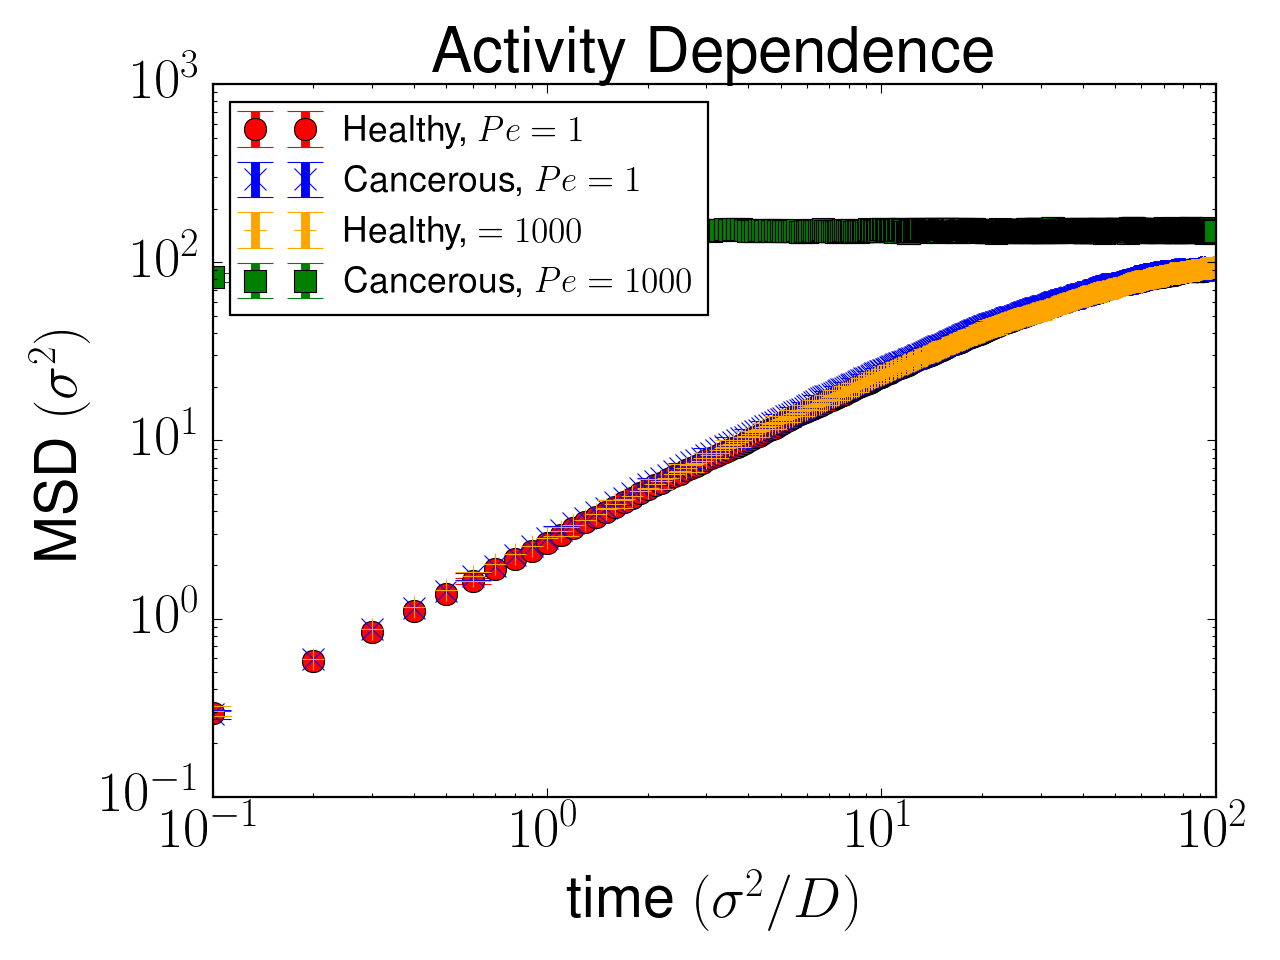
\includegraphics[width=1.0\columnwidth]{images/pe_both.png}
  \caption{The MSD for two different peclet numbers ($Pe$). The cancer cells and healthy cells have similar migratory behavior when the cancer cells have little self propulsion, $Pe=1$. Cancer cells are much more motile to begin with higher propulsion, $Pe=1000$, then reach a limit (when they are constrained by the boundaries).}
  \label{fig:prop}
\end{figure}


\subsubsection{Physiological Parameters}

The last set of parameters that the system was analyzed for was the physiologically relevant parameters.
These are the parameters mentioned prior: Cell stiffnesses of $2000Pa$ and $667Pa$ for healthy and cancer cells, respectively (or $1546$ and $510.6$ in dimensionless units), cancer cell propulsion of $12.5$ in dimensionless units, healthy cell adhesion of $1500$ in dimensionless units with an effective range of $0.2\sigma$, and a packing fraction of $0.7$.

The results compare closely with the behavior obsereved by collaborators in the lab.
The MSD (FIG. \ref{fig:phys} reveals that the cancer cells are more active than the healthy cells in the model, similiar to the behavior reported by the Wirtz group \cite{Lee}.
The segregation of the two systems also agrees with the experimental findings.
When cancer cells and healthy cells are mixed in a microfluidic droplet, the cancer cells are observed to migrate outwards while the healthy cells aggregate in the center \cite{Lu}.
The model produced qualitatively similiar results with identical behavior (See FIG. \ref{fig:separation}).


\begin{figure}
  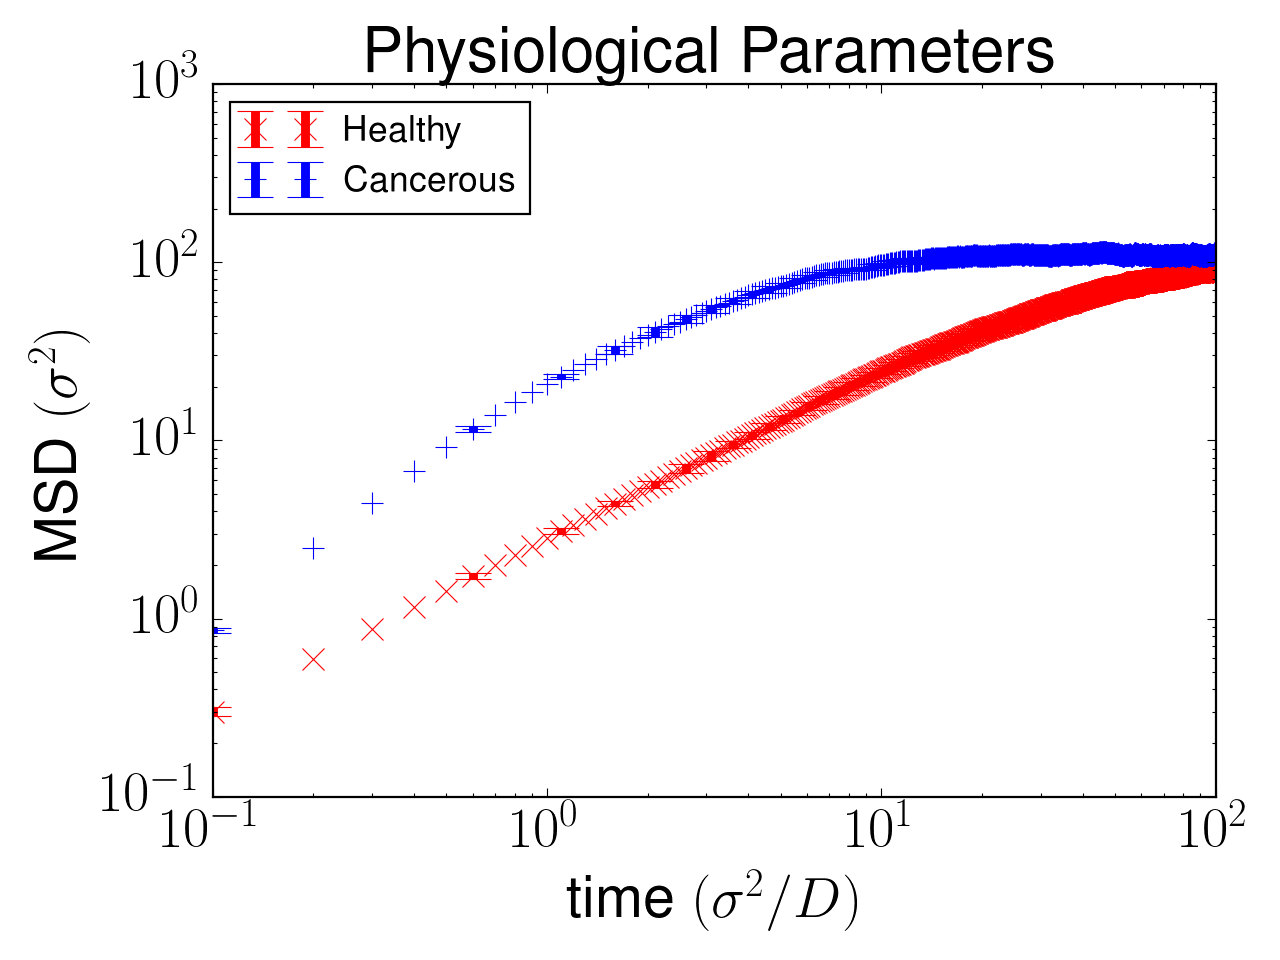
\includegraphics[width=0.9\columnwidth]{images/physmsd.png}
  \caption{The MSD for the cell co-culture for physiological parameters as mentioned in the text.}
   \label{fig:phys}
\end{figure}

\begin{figure*}
  \centering
  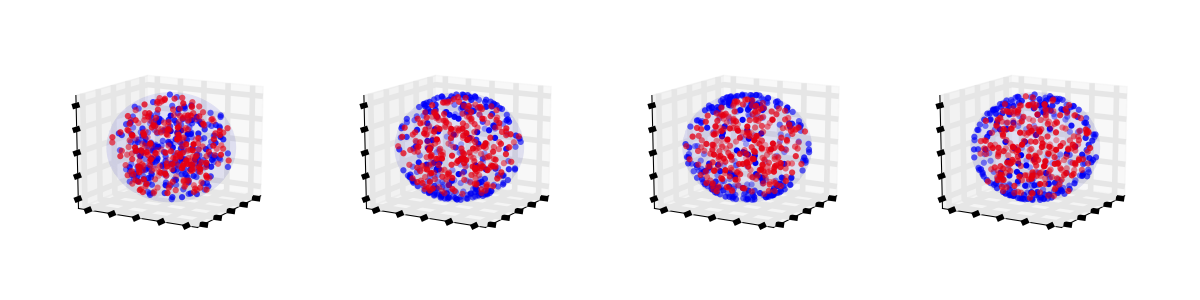
\includegraphics[width=\textwidth]{images/separation.png}
  \caption[separation]{Time evolution of the co-culture model of the cancer cells (Blue) and the healthy cells (Red) over a timescale of the order of seconds. The system evolves (left to right) from an initial, random state (left) towards a segregated state (right).}
   \label{fig:separation}
\end{figure*}


\section{Conclusions}
Over the course of capstone, I have created a robust, numerical model for co-culture colloids.
I studied the behavior of the model by testing many of its parameters and analyzing the behavior with regards to the migration and segragation of the different cell species.
I also applied parameters relevent to the physical case of healthy and cancer breast epithelial cells.
I began to compare the qualitative behavior of the model to experimental results and hope to soon make more absolute comparisons to quantitative measurements from our collaborators.
I began to also look at more complex variations of the parameters and the behavior they produce in the phase plane, though a more thorough analysis will have to wait for future work.

\begin{figure}
  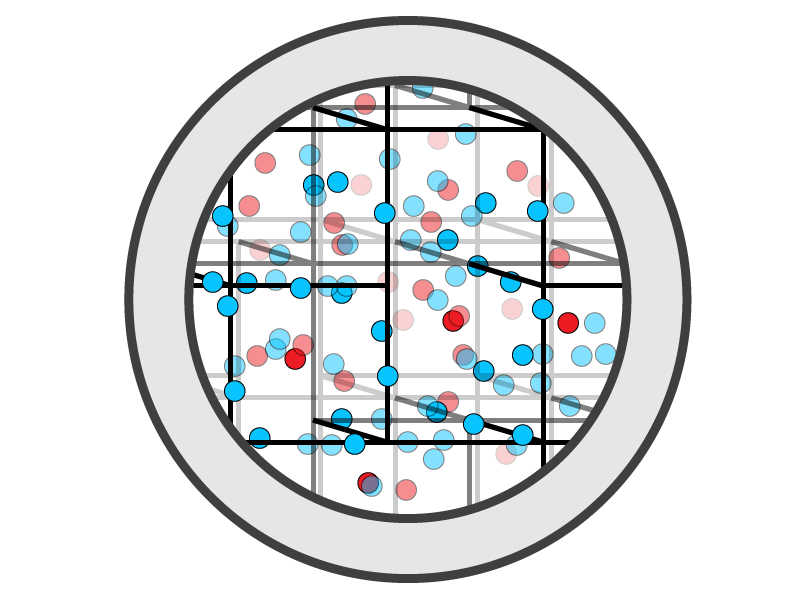
\includegraphics[width=0.9\columnwidth]{images/Fig2.png}
  \caption[capsuleECM]
   {A cross section of a spherical capsule enclosing a binary mixture of cells and an extracellular matrix.}
   \label{fig:capsuleECM}
\end{figure}

The qualitative behavior of the model has been compared to and found to match well with results from laboratory experiments.
However, a more direct comparison with quantitative results (like MSD) from the lab will be important for tuning the model to give physically accurate results.
This will hopefully be achieved through further, close collaboration with experimentalists and their data.

An investigation of the multi-dimensional parameter space was begun toward the end of the project, though it still needs to be examined more closely.
A detailed investigation of the parameter space of the model will prove to be difficult given the quantity of data needing to be produced for it.

Aside from further analysis of the model, there are also other components that may be added.
The model presented here was constructed using the minimal number of components necessary to produce qualitative behavior.
To make the model more rigorous, there are a couple suggested additions that might be made below:

\subsection{Interaction with the Extra Cellular Matrix}
The extracellular matrix (ECM) is a structural network of fibers that surrounds the cells (FIG. \ref{fig:capsuleECM}, and interacts with the contained cells \cite{Alberts}.
Most healthy cells adhere to the ECM and move along it in a manner mimicking one-dimensional motion \cite{Cukierman}.
Migration speed of cells in this manner has been observed to be significantly higher than on two dimensional surfaces \cite{Doyle}.
Considering the ECM and the interaction of cells with the ECM will thus be very important in the development of a complete model.
An ECM interaction with the cells could be modeled in the form of a disordered potential, or strands of static, adhesive particles.

\subsection{Cell Division}

The time scales that the migratory and segratory behavior is observed at is on the order of weeks \cite{Mingming}.
That time is sufficient enough for cell to divide several times and could have important effects on the behavior of the system.
The model could be made more sophisticated by accounting for cell division by duplicating cells after a specified period.

\begin{acknowledgments}
Many thanks to: Dr. Moumita Das for her mentorship and inputs, Julian Butcher for useful discussions, Drs. Minglin Ma and Mingming Wu for their collaboration and discussions, research computing at RIT for computational resources, and the Capstone Committee, especially Dr. Linda Barton, for their guidance and arranging of Capstone Program.
\end{acknowledgments}

\vspace{0.6in}
%
%change the name of the bibliography file to your own name
%make sure you have h-physrev5.bst file in the same directory as your tex file and bib file
%then compile using Latex-Bibtex-Latex-Latex sequence!
%

\bibliographystyle{h-physrev5.bst}
% now the actual bibliography file.   Note that it does not need the .bib extension in this line!
\bibliography{DanKolbmanBibliographyFile}
\end{document}

